%% Exemplo de utilizacao do estilo de formatacao normas-utf-tex (http://normas-utf-tex.sourceforge.net)
%% dúvidas acessar o site acima
%%
%%
%% Autores: (200?-2011) Hugo Vieira Neto (hvieir@utfpr.edu.br)
%%          (200?-2011) Diogo Rosa Kuiaski (diogo.kuiaski@gmail.com)
%%          (2011-2017) Marcos Talau <talau@users.sourceforge.net>
%% Colaborador:
%%          (2011) César M. Vargas Benitez <cesarvargasb@gmail.com>

%%
%% IMPORTANTE: O texto está escrito com acentuação antiga, atualmente você
%%             pode escrever acentos sem precisar de códigos para tal.
%%

\documentclass[openright]{normas-utf-tex} %openright = o capitulo comeca sempre em paginas impares
%\documentclass[oneside]{normas-utf-tex} %oneside = para dissertacoes com numero de paginas menor que 100 (apenas frente da folha) 

% force A4 paper format
\special{papersize=210mm,297mm}

\usepackage[alf,abnt-emphasize=bf,bibjustif,recuo=0cm, abnt-etal-cite=2, abnt-etal-list=99]{abntcite} %configuracao correta das referencias bibliograficas.

\usepackage[brazil]{babel} % pacote portugues brasileiro
\usepackage[utf8]{inputenc} % pacote para acentuacao direta
\usepackage{amsmath,amsfonts,amssymb} % pacote matematico
\usepackage{graphicx} % pacote grafico
\usepackage{times} % fonte times
\usepackage[final]{pdfpages} % adicao da ata
\usepackage{pgfplots}

%Podem utilizar GEOMETRY{...} para realizar pequenos ajustes das margens. Onde, left=esquerda, right=direita, top=superior, bottom=inferior. P.ex.:
%\geometry{left=3.0cm,right=1.5cm,top=4cm,bottom=1cm} 

% ---------- Preambulo ----------
\instituicao{Universidade Tecnológica Federal do Paraná} % nome da instituicao
\programa{DEPARTAMENTO ACADÊMICO DE ELETRÔNICA } % nome do programa
\area{ESPECIALIZAÇÃO EM INTERNET DAS COISAS} % [Engenharia Biom\'edica] ou [Inform\'atica Industrial] ou [Telem\'atica]

\documento{Dissertação} % [Disserta\c{c}\~ao] ou [Tese]
\nivel{Pos-graduação} % [Mestrado] ou [Doutorado]
\titulacao{Especialista} % [Mestre] ou [Doutor]

\titulo{{Sistema autônomo de gerenciamento de luzes}} % titulo do trabalho em portugues
\title{\MakeUppercase{Self-contained lighting management system}} % titulo do trabalho em ingles

\autor{Luis Denis Pliskievski de Lara} % autor do trabalho
\cita{LARA, Luis Denis Pliskievski de} % sobrenome (maiusculas), nome do autor do trabalho

\palavraschave{IOT, nodeMCU, ESP8266, energia, controle, autonomo} % palavras-chave do trabalho
\keywords{IOT, nomeMCU, ESP8266, energy, contro, self-contained} % palavras-chave do trabalho em ingles

\comentario{\UTFPRdocumentodata\ apresentada ao \UTFPRprogramadata\ da \ABNTinstituicaodata\ como requisito parcial para obtenção do grau de ``\UTFPRtitulacaodata\ em Intenet das Coisas Área de Concentração: \UTFPRareadata.}

    \orientador{Prof. Glauber Gomes de Oliveira Brante} % nome do orientador do trabalho
%\orientador[Orientadora:]{Nome da Orientadora} % <- no caso de orientadora, usar esta sintaxe
%\coorientador{Nome do Co-orientador} % nome do co-orientador do trabalho, caso exista
%\coorientador[Co-orientadora:]{Nome da Co-orientadora} % <- no caso de co-orientadora, usar esta sintaxe
%\coorientador[Co-orientadores:]{Nome do Co-orientador} % no caso de 2 co-orientadores, usar esta sintaxe
%\coorientadorb{Nome do Co-orientador 2}	% este comando inclui o nome do 2o co-orientador

\local{Curitiba} % cidade
\data{\the\year} % ano automatico

% desativa hifenizacao mantendo o texto justificado.
% thanks to Emilio C. G. Wille
\tolerance=1
\emergencystretch=\maxdimen
\hyphenpenalty=10000
\hbadness=10000
\sloppy

%---------- Inicio do Documento ----------
\begin{document}

\capa % geracao automatica da capa
\folhaderosto % geracao automatica da folha de rosto

% Lembre-se de que a ficha catalografica eh impressa no verso da folha de rosto
% Ficha catalografica
\fichacatpum{T137}
\fichacatautor{Lara, Luis Denis Pliskievski de}
\fichacatpgbib{\pageref{bibstart}-\pageref{bibend}}
\fichacatpalcha{1. Intenet das coisas. 2. Redes de comutadores. 3. TCP/IP (Protocolo de rede de computação), ...}
\fichacatpdois{CDD (22. ed.) 621.3}
\fichacatbib{Biblioteca xxxxxx}
\fichacat

% insercao da ATA
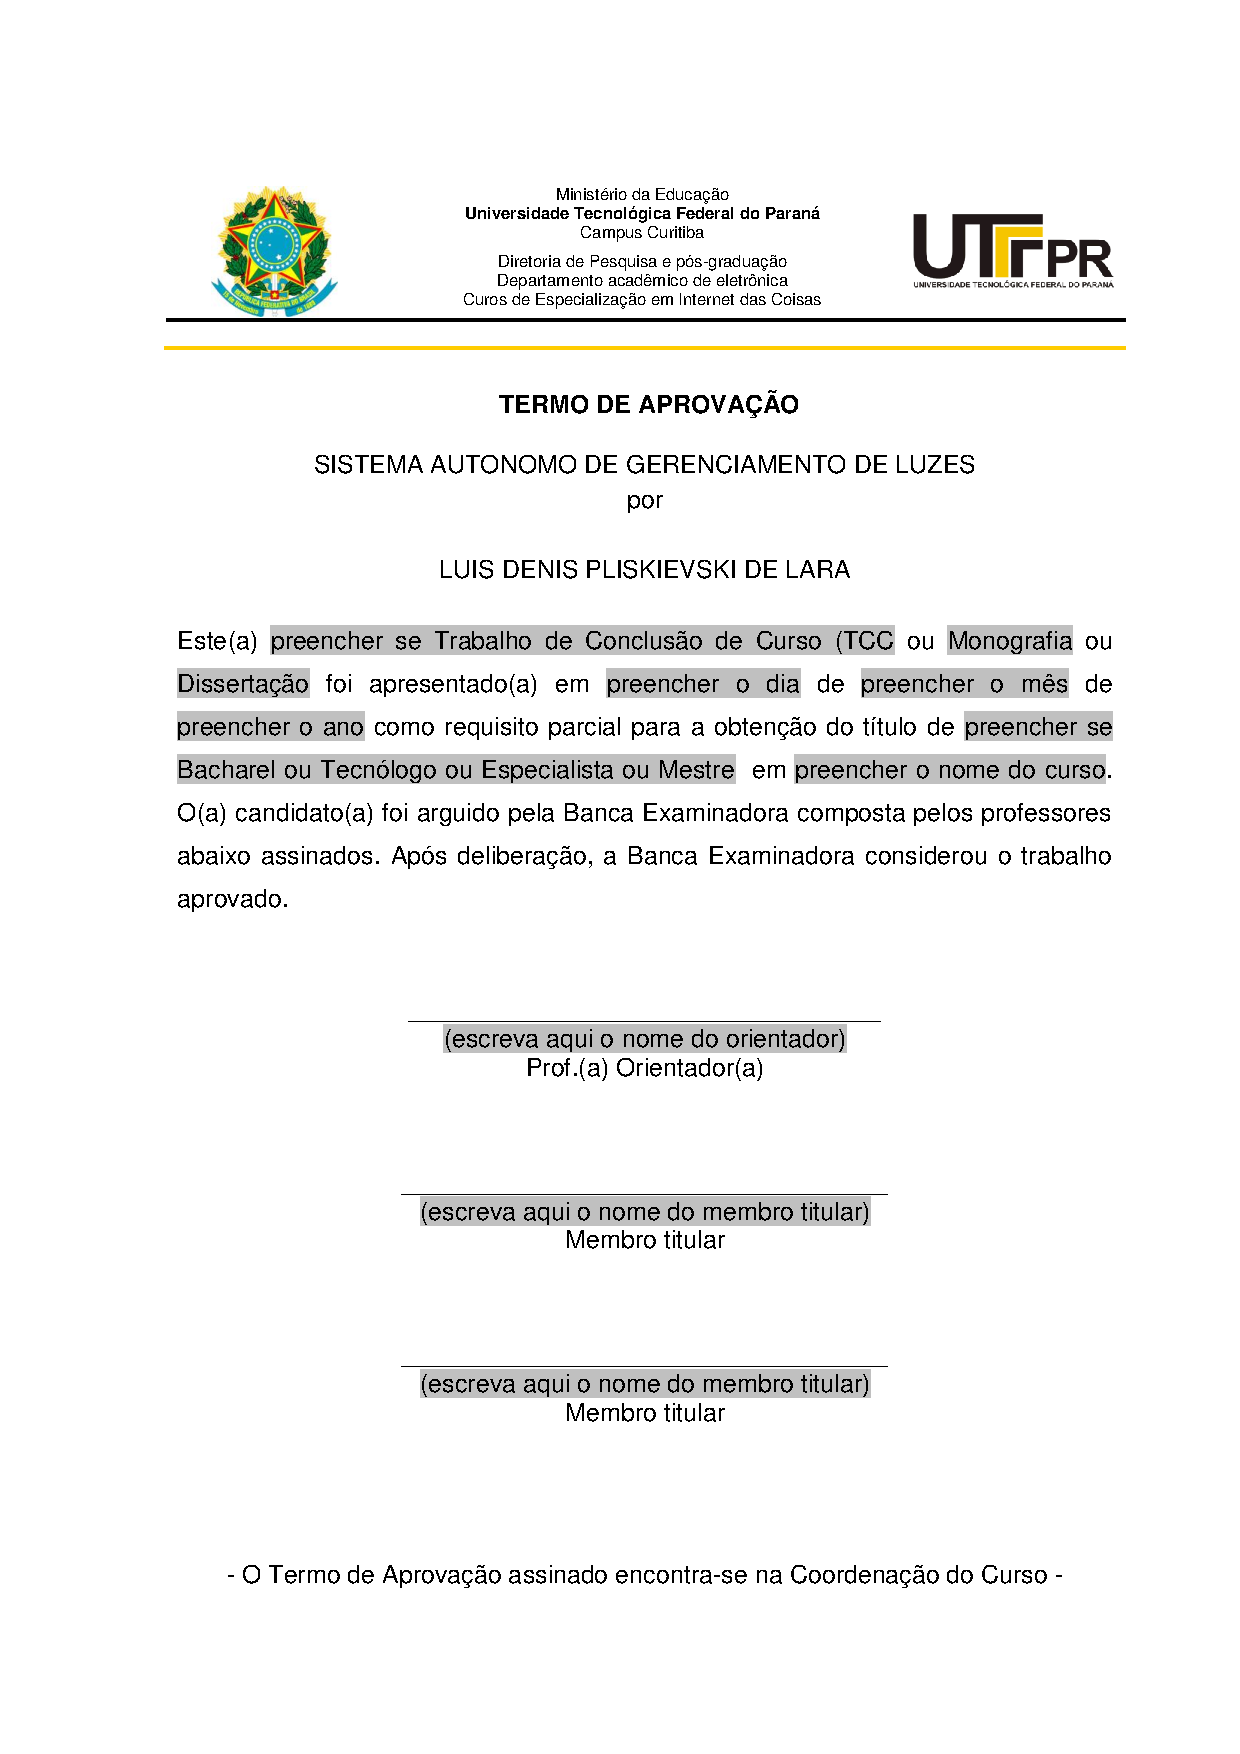
\includepdf{termo.pdf}

% dedicatoria
\begin{dedicatoria}
Dedico esse trabalho em memória de minha mãe que sempre me incentivou a buscar mais conhecimento.
\end{dedicatoria}

% agradecimentos (opcional)
\begin{agradecimentos}
A todos que de alguma forma me apoiaram na trajetoria, não deixaram eu desistir e mais do que nunca acreditaram em mim em momentos que eu dúvidava da minha capacidade.
Agradeço ao meu colega Konrado Biernet por me ajudar a desenvolver esse trabalho e a minha namorada Aline Frassato, por compreender os tempos que tive que deixa-la sozinha.
\end{agradecimentos}

%resumo
\begin{resumo}
Essa dissertação mostra de forma prática o uso da internet da coisas para buscar eficiência no uso de recursos energéticos voltados para gerenciamento de luzes, ponto aonde temos um gasto substâncial e muitas vezes mal administrado.

Para o desenvolvimento usamos insumos facilmente encontrados no mercado local além de ótimas documentações e casos de uso, o que facilitou a prototipagem do projeto. Durante a programação das funções foram encontradas algumas situações adversas que citamos no capítulo de desenvolvimento. 

No início do projeto a meta era uma redução do consumo na casa de 7\%, mas os resultados encontramos foram mais eficiêntes que o previsto.

\end{resumo}

%abstract
\begin{abstract}
This dissertation shows in a practical way the use of the internet of things for the search of efficiency in the use of energy resources directed to the management of light, and today we have a specific and often mismanaged expense.access.

For the development we use inputs easily found in the local market besides great documentation and use cases, which facilitated the prototyping of the project. During the programming of the functions were found some adverse situations that we mentioned in the chapter of development.

At the beginning of the project the goal was to reduce consumption by 7 \%, but the results we found were more efficient than expected.
\end{abstract}

% listas (opcionais, mas recomenda-se a partir de 5 elementos)
%\listadesiglas % geracao automatica da lista de siglasp
\listadefiguras % geracao automatica da lista de figuras
%\listadequadros % adivinhe :)
%\listadesiglas


% sumario
\sumario % geracao automatica do sumario


\setcounter{page}{12}

%---------- Primeiro Capitulo ----------

\chapter{Introdução}


Com o advento da internet e evolução, temos a possibilidade de criar dispositivos inteligentes \cite{Novatec} para nos auxiliar em situações corriqueiras, como controle de acesso, controle de frotas, gerenciamento de energia e água.

Um estudo apresentado pela empresa Vodafone \cite{Vodafone} mostra que 84\%  das empresas pequenas ou grandes afirmam que o uso da internet das coisas cresceu em suas estruturas apresentam  um  percentual 95\% de resultados tangíves.

Outro estudo apresentado pela Logicallis \cite{Logicallis}, mostra que para 81\% das empresas o uso de IOT será muito importante para os negócios nós próximas 3 à 5 anos. Para muitos executivos a maturidade das tecnologias apresentadas transformam as tecnologias de Internet das Coisas ficam de alta ou muito alta a importância do uso das técnologias em seus seus negôcios. Segundo o mesmo estudo a eficiência de cerca de 18\% em resultados, aonde são aplicadas as soluções  é o principal benefício para justificar sua implantação \cite{IotSnapshot}.
 
Para fomentar o desenvolvimento de tecnologia o Banco Nacional de Desenvolvimento  e o Ministério da Ciência, Tecnologia, Inovações e Comunicações  apresentaram em 2017 o Estudo Nacional de Internet das Coisas, aonde os estudos estarão concentrandos nas áreas de cidades inteligentes, saúde, industria e agronegócios\cite{BNDES}.
 
Sabendo que em todos os estabelecimentos comerciais e residências utilizam energia elétrica e o seu uso tem uma grande representativade no orçamento mensal. Tendo em  consideração a necessidade de uma ação humana para interação com luzes (ligar/desligar), temos um grande desperdício com esquecimentos de luzes acessas em lugares não usados.

Nesse trabalho iremos desmostrar um sistema inteligente de gerenciamento de luzes para comércio, empresas e mesmo casas. Alinhando assim a tecnologia com o uso consciênte de energia elétrica, trazendo maior eficiência no consumo e de contra partinda uma redução de custos.

\section{Motivação}

Hoje temos um grande desperdicio de energia mantendo luzes acessas em lugares que não estão sendo usados, como sala de reunião, banheiros, iluminação ornamental, luzes internas e externas.

A ideia com o uso desse dispositivo é mensurar o consumo e mostrar através de números a diferença de gastos, quando usamos de forma consciênte a energia, facilitando a tomada de decisão para a administração e também expandir o estudo futuramente sobre o controle sobre outros meios de consumo de energia, planejanto ambientes inteligêntes, baseando em efiência energética.

\section{Objetivos}

\subsection{Objetivo Geral}

A ideia principal é conseguir mostrar através de gráficos e números o quanto é possível economizar e tornar-se mais eficiente na questão de gastos referente a utilização de energia elétrica.

Ser uma ferramenta que auxilia no gerenciamento de gastos do estabelecimento, trazer previsões e manter históricos de consumo, afim de gerar informações para tomadas de decisão futuras.

\subsection{Objetivos Específicos}

\begin{itemize}
	\item Controlar o consumo de energia.
	\item Representar por meio de números o consumo real. 
	\item Melhorar o consumo energético através de gerenciamento autonomo.
	\item Entregar uma previsão de consumo x gasto mensal.
\end{itemize}


%---------- Segundo Capitulo ----------
\chapter{Desenvolvimento}
\label{chap:desenv}

 
Para o desenvolvimento do firmware do projeto foi utilizando a linguagem C++   \cite{Altabooks} e recursos HTTP.

Os insumos utilizados para o desenvolvimento do protótipo para testes foram:

\begin{itemize}
       	\item ESP8266 - NomeMCU V3
        \item Sensor de corrente Allegro ACS712 (ACS712ELCTR-30A-)
        \item Servidor MQTT
        \item Sensor de presença PIR DYP-ME003
\end{itemize}

A seguir vamos apresentar algumas especificações técnicas dos recursos utilizados para o desenvolvimento do projeto.

Essas dados foram utilizadas como base na tomada de decisão sobre o uso dos insumos. 

\section{NodeMCU}
Ao realizar uma busca em qualquer sitio de busca on-line, encontramos uma grande quantidade referências ao módulo NodeMCU (ESP8266).

Esse módulo se mostrou uma boa opção, devido ao requisitos técnicos listados abaixo.

\begin{itemize}
    \item Certificação WIFI Alliance;  \cite{espressif}
    \item Protocolos 802.11 b/g/n;\cite{espressif}
    \item CPU Tensilica L106 32-bit processor (80MHz ~ 160MHz )  \cite{Novatec}
    \item 4MB de armazenamento;
    \item Suporte aos modos Station/SoftAP/SoftAP+Station;\cite{espressif}
    \item Autenticação WEP/WPA/WPA2 com encriptação TKIP/AES;\cite{espressif}
    \item Suporte atualização OTA;\cite{espressif}
    \item Protocolos de Rede IPv4, TCP/UDP/HTTP;\cite{espressif}
\end{itemize}

Abaixo uma imagem mostrando o hardware.

\begin{figure}[h!b]
\centering 
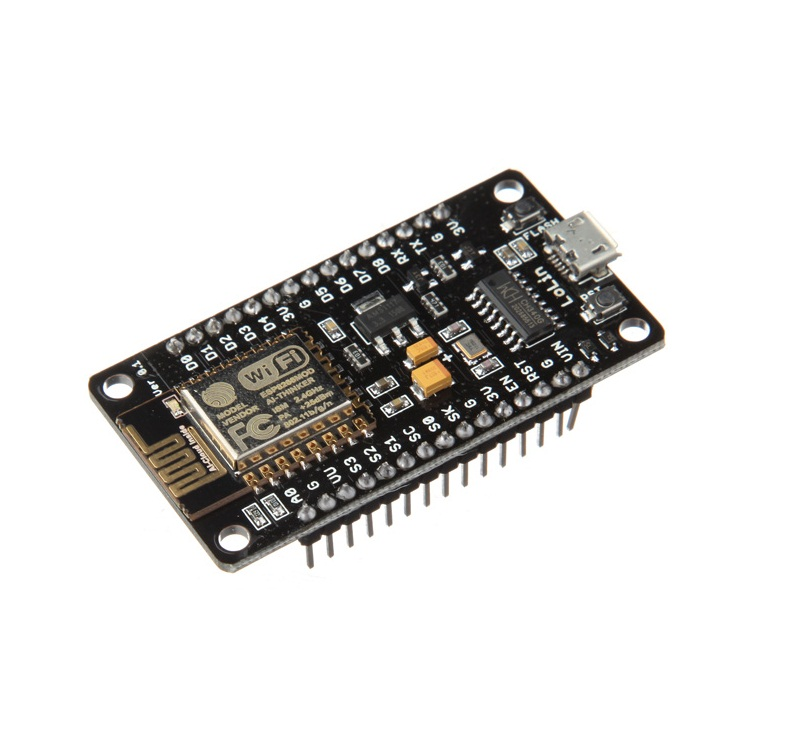
\includegraphics[scale=0.5]{nodemcu.jpg}
\caption{NodeMCU V3}
\label{NodeMCU}
\end{figure}

Durante o processo de desenvolvimento, identificamos uma limitação quanto ao número de conexões simultaneas a um único NodeMCU. 

Não foi possível estabelecer mais que 5 conexões simultâneas, quando a sexta conexão era estabelecida, a mais antiga era perdida, algo que não foi possível contornar no momento.

\section{Sensor de corrente Allegro ACS712}
O medidor de corrente Allegro ACS712  \cite{Allegro} pode trabalhar com correntes de -30A à +30A   \cite{Allegro} , mais que suficiente para os padrões que usamos em estrutura de iluminação, aonde as correntes geralmente não são maiores que 10A. A seguir uma imagem do sensor, com a conexão de leitura.

\begin{figure}[!htb]
     \centering
     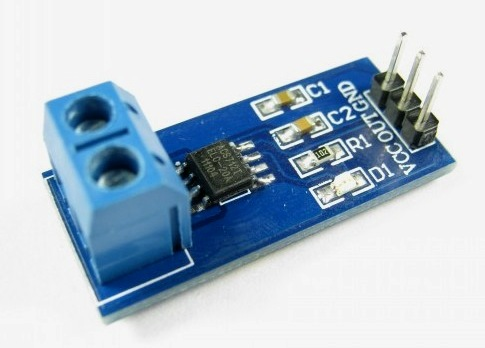
\includegraphics[scale=0.6]{AllegroACS712.jpg}
     \caption{Allegro ACS712}
     \label{fig:AllegreoACS712}
\end{figure}

Como o sensor é invasivo, temos uma melhor leitura dos dados, gerando dados mais fidedignos ao consumo real.

A taxa de amostragem durante o desenvolvimento teve uma pequena diferença se comparando com o resultado de um multímetro. Essa diferença ficou entre 55mA e 70mA. Isso acontece devido ao ruído do processador L106 e o ruído do próprio Allegro ACS712.
 
\section{Sensor de presença PIR DYP-ME003}

Também utilizamos um sensor de presença modelo PIR DYP-ME003   \cite{openimpulse}
para ter um controle automático da ação de acender e apagar as luzes da sala.

A abaixo uma imagem ilustrativa do dispostivo:
\begin{figure}[!htb]
     \centering
     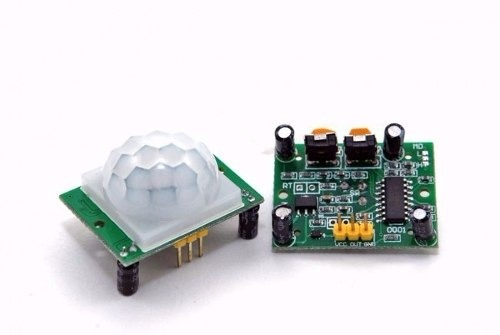
\includegraphics[scale=0.6]{PIR.jpg}
     \caption{PIR DYP-ME003}
     \label{fig:PIR DYP-ME003}
\end{figure}

O dispositivo oferece algumas caracteristicas interessantes ao projeto, como:

\begin{itemize}
    \item Distância ajustável com precisão até 7 metros;
    \item Atraso de envio de pulso ajustável entre 5 e 200 ms;
\end{itemize}

Com isso no momento que a pessoa entra da sala o sensor envia um sinal  via GPIO,  acendendo as lâmpadas automaticamente e inicializa também a bilhetagem do consumo da sala.

\section{Firmware}

Para desenvolvermos o firmware usamos a linguagem C++ \cite{Altabooks}. 

Ao ligar o equipamento teremos uma flag booleana \cite{Elsevier}, que irá nos dizer se é ou não a primeira inicialização do dispositivo, conforme podemos ver no fluxo a seguir:

\begin{figure}[!htb]
     \centering
     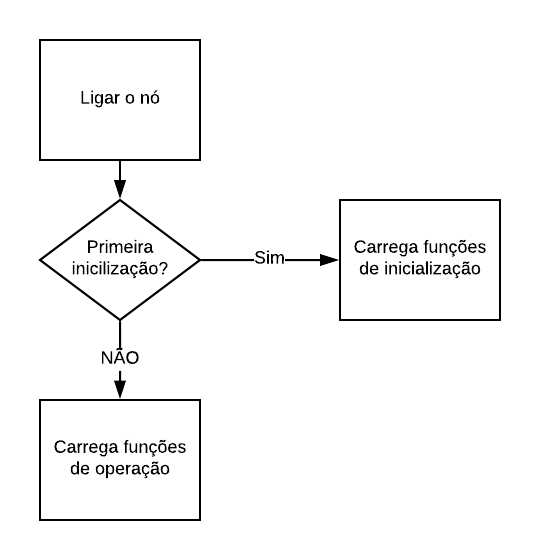
\includegraphics[scale=1]{Primeira_Inicializacao.png}
     \caption{Fluxo Inicialização}
     \label{}
\end{figure}

O software está divido basicamente em duas frentes,

\begin{itemize}
    \item Primeira Inicialização e configuração primária;
\end{itemize}
A segunda parte, Gerenciador de Funções, tem subfunções para realizar as ações necessárias.
\begin{itemize}
    \item Gerenciador de funções;
    \subitem Controle de Luzes;
    \subitem Verificado de Luzes;
    \subitem Intensidade;
    \subitem Consumo;
    \subitem Verificar Grupos;
    \subitem Trocar de Grupo;
    \subitem Respostas Autônomas;
    \subitem Atualização OTA;
\end{itemize}

O firmware foi divido em 2 partes para facilitar o entendimento do funcionamento básico, mas em tempo real é executado somente um binário.

Para a troca de mensagens definimos um formato JSON \cite{json-devmedia}. Esse formato permite a troca de mensagens de forma simples e sem exigir redes de alto desempenho para garantir uma entrega dos dados.

O leiaute básico do JSON é:

\begin{center}
\textit
sensor\{\\ 
status: boolena; \\
dimmer: int16;\\
Consumo:int16; \\
grupo:string;\\
laststate: boolean;\\
Hearbeat: date: \\
PresenceSensor:boolean:\\
\}
\end{center}
\subsection{Primeira Inicialização e configuração primaria}


Na primeira inicialização do dispositivo, o rádio será configurado como AP e terá um servidor DHCP para fornecer 2 IP's classe C.

Com isso podemos utilizar um notebook ou smartphone para abrir a página de configuração do dispositivo.

Há  um servidor WEB com acesso via porta 80 e a uma página HTTP que será utilizada para configurar os dados de forma clara, pois a página não terá abas ou outras páginas de navegação.

Na página de configuração poderes setar as seguintes opções:
\begin{itemize}
    \item Nome do dispositivo;
    \item Grupo do dispositivo;
    \item Nome da Rede;
    \item Senha de acesso;
    \item Tipo de autenticação e padrão criptografia;
    \item Habilitar ou desabilitar o acesso via SSH;
\end{itemize}

Em caso de falha na configuração ou qualquer outra situação, existe um botão de reset, que através de uma GPIO \cite{Elsevier} realizar um limpeza nos parâmetros e seta a variavel booleana de inicio para verdade, com isso o firmware retorna o estado de fábrica, podemos assim realizar todo o processo de configuração novamente.

Abaixo o fluxo de inicialização e configuração do dispositivo.
\begin{figure}[!htb]
     \centering
     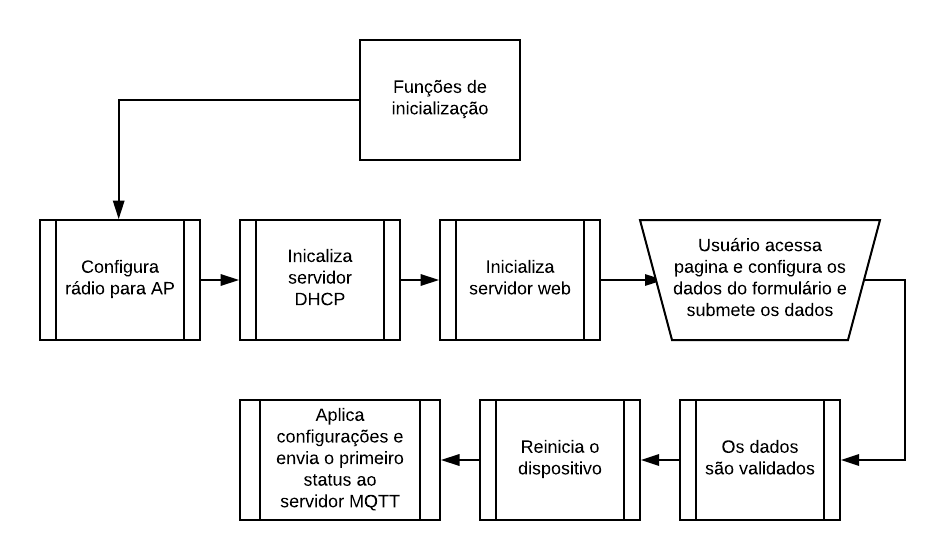
\includegraphics[scale=1]{Ini_flux.png}
     \caption{Processo de inicialização e gravação dos dados iniciais}
     \label{}
\end{figure}

\subsection{Gerenciador de funções}

A integração com o serviço de fron-end é realizado através de servidor MQTT \cite{Novatec}. Através desse servidor são replicadas as configurações e informações capturadas durante o uso do dispositivo. 

O firmware ao receber uma mensagem da plataforma via MQTT, válida se o comando solicitado existe e direciona para sua função específica. Caso seja recebido algum valor inválido, é retorna um NACK.

Abaixo as opções disponíveis, bem seu respectivo byte de controle:

\begin{itemize}
    \item Acender/Apagar luz = 0x02;
    \item Estado na Luz=0x03;
    \item Controlar intensidade da Luz = 0x04;
    \item Consumo = 0x05;
    \item Verificar grupo 0x06;
    \item Trocar de grupo = 0x07;
    \item Respostas autônomas 0x08;
\end{itemize}

O fluxo abaixo exibe de forma sucinta o fluxo do gerenciador de funções.

\begin{figure}[!htb]
     \centering
     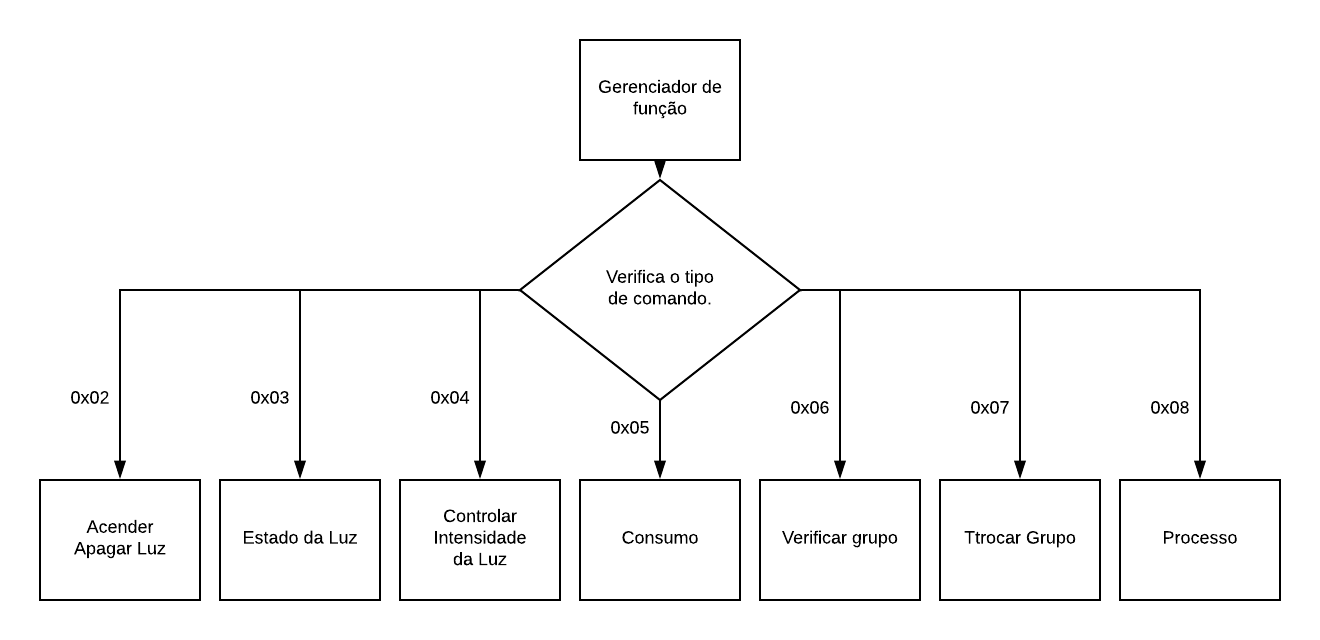
\includegraphics[scale=0.7]{3_flux.png}
     \caption{Gerenciador de funções}
     \label{}
\end{figure}


\subsubsection{Acender/Apagar luz}

Ao receber o byte 0x02 via servidor verificamos se o parâmetro necessário foi passado corretamente. A função espera receber um valor INT com valores 0 ou 1.

Caso a interação seja via GPIO, o firmware irá montar a mensagem e passar os valores corretos a função para que seja realizada a ação esperada.

Os parâmetros esperados são:
\begin{itemize}
    \item O - Apaga a luz;
    \item 1 - Acende a luz;
\end{itemize}

Antes de executar a ação é verificado o estado atual do dispositivo, e a função é executada somente se o estado atual for diferente do novo estado recebido.

Se o comando for executado com sucesso será enviado uma resposta de ACK para o gerenciador remoto, caso contrário o mesmo receberá um NACK.

Se o parâmetro informado for inválido, será retornado um NACK.

\subsubsection{Estado na Luz}

No momento que o firmware receber o byte de controle 0x03, irá retornar o estado atual das luz no formado binário aonde:

\begin{itemize}
    \item O - Luz apagada;
    \item 1 - Luz acessa;
\end{itemize}

\subsubsection{Controlar intensidade da Luz}
A função para controlar a intesidade de luz tem como definição byte 0x04, e tem como parâmetro uma váriavel int que deve ter o valor entre 2 e 99.

Ao receber esse valor é aplicado então sobre as luzes um dimmer, para mudar a intesidade da luz. O valor recebido é aplicado em formato de porcentagem.

No exemplo abaixo, recebemos uma mensagem 0x04 com o parâmetro 50. Então será aplicado a luz 50\% de intensidade.

\begin{center}
    \textit{
    Luz =  50\%
    }
\end{center}

Antes de executar a ação é verificado o estado atual do dispositivo, e a função é executada somente se o estado atual for diferente do novo estado esperado.

Se função receber algum valor fora do padrão delimitado, será enviado uma resposta de NACK para o servidor.

\subsubsection{Consumo}
O receber o byte de controle 0x05, verificamos o estado do dispositivo, se o mesmo está ligado, consultamos o valor de consumo e retornamos para aplicação.

O retorno terá o total de consumo e minutos de utilização até o momento.

Caso a luz esteja apagada no momento da solitação, será retornado o valor 0 (zero) para aplicação.

O valor das variáveis são zeradas somente no momento que o dispositivo é desligado, nesse momento o valor é enviado o servidor e gravado em um banco de dados local, aonde sempre teremos os dois ultimos dados medidos;

\subsubsection{Verifica grupos}

Ao receber uma mensagem 0x06, o dispositivo irá retornar os seguintes valores:

\begin{itemize}
    \item Nome do dispositivo;
    \item Grupo do dispositivo;
    \item Nome da Rede utilizada;
    \item Intensidade de sinal;
    \item Data-hora do dispositivo;
    \item Valor sensor de presença;
\end{itemize}

\subsubsection{Trocar de Grupo}
Ao receber a mensagem 0x07 para troca de grupo o dispositivo irá verificar se o grupo atual e igual ao novo grupo recebido, caso seja diferente aplicará o novo ao dispositivo.
A função espera uma váriavel string\cite{Altabooks} como parâmetro.
Exemplo:
\begin{center}
    \textit{
    0x07 "grupo 2"
    }
\end{center}

Não é necessário reiniciar o dispositivo para aplicar o novo grupo.

\subsubsection{Respostas autônomas}

Foi criada uma ação autônoma para enviar os dados de consumo, sempre que as luzes estiverem acessas. 

Serão enviados dados de consumo a cada 45 segundos, com as seguintes informações:

\begin{itemize}
    \item Nome do dispositivo;
    \item Valor Consumo;
    \item Tempo de uso;
\end{itemize}

A cada ação recebida via MQTT ou GPIO,  envia uma mensagem para servidor com os seguintes dados;

\begin{itemize}
    \item Nome do dispositivo;
    \item IP do dispositivo;
    \item Mascará de rede;
    \item gateway padrão;
    \item Valor estado;
    \item Valor dimmer;
    \item Valor Consumo;
    \item Grupo;
    \item Ultimo estado;
    \item Data-hora do dispositivo;
    \item Valor sensor de presença;
    \item Tempo em atividade;
    \item Versão do firmware;
\end{itemize}

\subsection{Atualização OTA}

O NodeMCU suporta atualização de firmware via rede wireless  \cite{espressif}, sendo assim não é preciso conectar um cabo usb para realizar o processo no mesmo. 
Pensando nessa funcionalidade crei uma função para receber o firmeare a fazer a atualização.

Ao receber a mensagem de atualizaçao disponível é comparada a versão local com a nova versão, caso sejam diferentes o dispositivo conecta-se a um repositório e realiza a cópia do novo arquivo, uma vez realizada a cópia, é checada a integridade através de uma comparação entre o  MD5 do servidor com o hah MD5 do arquivo local, se a combinação for igual dos MD5, então para os serviços são parados e é realizado uma cópia de backup do binário, e então aplicado o novo arquivo.

Após a atualização do firmware não é necessário reconfigurar o dispositivo, pois as configurações são salvas em uma parte segregada da memória e a leitura é realizada de forma automática pelo firmware.

\section{Cenário de testes}
Realizamos os testes durante 5 dias em duas salas de reunião. A salas ficam em um prédio comercial aonde as luzes são acessas todos os dias às 7 horas da manhã e são delisgadas às 19 horas.

No local não havia a politica de desligar as luzes em momento de ociosidade da sala, ou seja a luz permanecia acessa do início da manhã até o início da noite, independente de estar sendo usada ou não. 

Na sala 1 não foi instalado o dispositivo, já na sala 2 o dispositivo ficou operacional por 5 dias.

Foram 120 horas de amostras coletadas durante esse periodo, dessas 120 horas, temos 60 horas da sala 1 e mais 60 horas da sala 2.

Durante os testes tivemos uma economia próxima de 43\%, mas essa diferença se deu devido ao seguintes fatos. 

\begin{itemize}
    \item Das 7 às 8 e das 18 às 19 não são realizadas reuniões;
    \item Entre 12 e 13:30 a sala também não é utilizada;
\end{itemize}

Excluíndo esse cenário, no pior cenário teríamos um ganho de eficiêcia de 28,22\% em média por sala de reunião.

No gráfico a seguir podemos ver de forma clara a diferença de consumo entre a sala gerenciada automaticamente e a sala sem o controle autônomo. 

\begin{figure}[!htb]
     \centering
     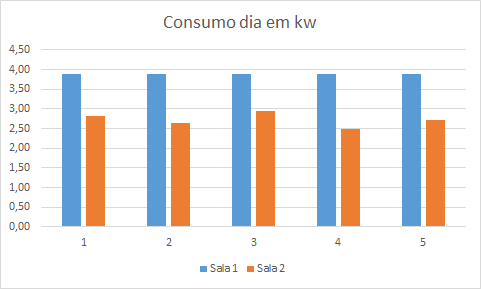
\includegraphics[scale=0.8]{g2.png}
     \caption{Diferença de consumo entre salas 1 e 2}
     \label{}
\end{figure}




%---------- Terceiro Capitulo ----------
\chapter{Conclusão}

Vemos que a utilização dos recursos de IOT podem nos ajudar no gerenciamento de energia, como nesse caso aplicado à luzes, mas podendo ser ampliado para qualquer cénario que utilize energia elétrica como recurso principal.

Com o decorrer do desenvolvimento do trabalho, conseguimos notar o quanto disperdiçamos a energia elétrica, muitas vezes de forma inconsciente.   

As soluções de IOT trazem para nosso o cotidiano forma de automatizar decisões simples, que muitas vezes pela correria do dia a dia não conseguimos tomar ou mesmo não executamos por força do hábito. 

Com a automatização de pequenas decisões, como apagar uma luz, desativar a energia de alguns pontos, podemos além usar os recursos com mais eficiência, podemos gerar uma redução de custo considerável, como no exemplo aplicado durante o desenvolvimento aonde conseguimos uma redução de até 23\%, essa diferença pode represetar um valor significativo para grandes corporações, prédios publicos ou mesmo residências.

Com a crescendo de acesso a conexões e diminuição do custo de desenvolvimento de hardware, em um futuro próximo poderemos ter automatizações como essas em todo tipo de prédio sem gerar maiores gastos para sua implantação, abrindo de forma abrangente o mercado para novas empresas e novas soluções de gerenciamento.

Mostrando assim que temos uma mercado a ser explorado com grande potêncial de crescimento a médio e longo prazo.

\label{bibstart}
\bibliography{reflatex} % geracao automatica das referencias a partir do arquivo reflatex.bib
\label{bibend}

% --------- Ordenacao Afabetica da Lista de siglas --------
%\textbf{* Observa\c{c}\~oes:} a ordenacao alfabetica da lista de siglas ainda nao eh realizada de forma automatica, porem
% eh possivel se de realizar isto manualmente. Duas formas:
%
% ** Primeira forma)
%    A ordenacao eh feita com o auxilio do comando 'sort', disponivel em qualquer
% sistema Linux e UNIX, e tambem em sistemas Windows se instalado o coreutils (http://gnuwin32.sourceforge.net/packages/coreutils.htm)
% comandos para compilar e ordenar, supondo que seu arquivo se chame 'dissertacao.tex':
%
%      $ latex dissertacao
%      $ bibtex dissertacao && latex dissertacao
%      $ latex dissertacao
%      $ sort dissertacao.lsg > dissertacao.lsg.tmp
%      $ mv dissertacao.lsg.tmp dissertacao.lsg
%      $ latex dissertacao
%      $ dvipdf dissertacao.dvi
%
%
% ** Segunda forma)
%\textbf{Sugest\~ao:} crie outro arquivo .tex para siglas e utilize o comando \sigla{sigla}{descri\c{c}\~ao}.
%Para incluir este arquivo no final do arquivo, utilize o comando \input{arquivo.tex}.
%Assim, Todas as siglas serao geradas na ultima pagina. Entao, devera excluir a ultima pagina da versao final do arquivo
% PDF do seu documento.


%-------- Citacoes ---------
% - Utilize o comando   \citeonline{...} para citacoes com o seguinte formato: Autor et al. (2011).
% Este tipo de formato eh utilizado no comeco do paragrafo. P.ex.:   \citeonline{autor2011}

% - Utilize o comando   \cite{...} para citacoeses no meio ou final do paragrafo. P.ex.:   \cite{autor2011}



%-------- Titulos com nomes cientificos (titulo, capitulos e secoes) ----------
% Regra para escrita de nomes cientificos:
% Os nomes devem ser escritos em italico, 
%a primeira letra do primeiro nome deve ser em maiusculo e o restante em minusculo (inclusive a primeira letra do segundo nome).
% VEJA os exemplos abaixo.
% 
% 1) voce nao quer que a secao fique com uppercase (caixa alta) automaticamente:
%\section[nouppercase]{\MakeUppercase{Estudo dos efeitos da radiacao ultravioleta C e TFD em celulas de} {\textit{Saccharomyces boulardii}}
%
% 2) por padrao os cases (maiusculas/minuscula) sao ajustados automaticamente, voce nao precisa usar makeuppercase e afins.
% \section{Introducao} % a introducao sera posta no texto como INTRODUCAO, automaticamente, como a norma indica.


\end{document}

